\documentclass{article}
\usepackage{iclr2026_conference,times}
\input{math_commands.tex}

\usepackage{hyperref}
\usepackage{url}
\usepackage{booktabs}
\usepackage{array}
\usepackage{graphicx}
\newcommand{\score}[2]{#1{\scriptsize$\pm$#2}}

\title{Semantic-Structural Robust Propagation for GNNs}

\author{Internal Research Memo \\
Working draft for discussion}

\iclrfinalcopy
\begin{document}
\onecolumn
\maketitle

\begin{abstract}
Internal technical memo. This document records the current problem framing,
threat model, RUNG backbone, semantic trust mechanisms, and preliminary
results for discussion.
\end{abstract}

\section{Problem and Motivation}

Consider node classification on a text-attributed graph $G=(V,E)$. A standard
message-passing layer updates a node by aggregating messages from its observed
neighbors:
\[
  h_i^{(\ell+1)} \leftarrow
  \mathrm{Update}\!\left(h_i^{(\ell)},
  \mathrm{Aggregate}\bigl(\{h_j^{(\ell)}:j\in N(i)\}\bigr)\right).
\]

This computation assumes that the observed neighborhood provides reliable
evidence. In practice, graphs can contain noisy, incorrect, or adversarially
injected edges that transport misleading messages.

At each robust message-passing update, the model must make two decisions:
\begin{enumerate}
  \item \textbf{How much influence should the aggregate neighborhood message
  have?}
  \item \textbf{How should that influence be distributed across individual
  neighbors?}
\end{enumerate}

To make these decisions on an unreliable graph, the model has access to two
different sources of evidence: \textbf{graph-internal dynamic evidence}, such
as topology and evolving node representations, and \textbf{graph-external
relation semantics}, inferred from original node texts. Structural evidence
alone can be fooled by camouflaged edges, while semantic evidence alone cannot
fully characterize the current propagation state.

Existing robust GNNs typically answer both decisions using graph-internal
signals, such as topology, feature similarity, or evolving representations.
Our current v3 design makes one explicit division of labor: RUNG uses dynamic
graph-internal evidence to estimate the overall neighborhood influence, while
the LLM uses graph-external relation semantics to allocate that influence
across neighbors.

\paragraph{Research question.}
How can we combine structural robustness and relation semantics for reliable
message passing on unreliable graphs?

\section{Threat Model: Text-Camouflaged Edge Injection}

\paragraph{Attacker capability.}
The attacker knows the victim model and can add edges before evaluation, but
cannot modify node texts.

\paragraph{Candidate generation.}
The attacker first retrieves textually related non-neighbor pairs, then uses
white-box projected gradient descent (PGD) to select the subset of edges that
maximally degrades node classification.

\paragraph{Key asymmetry.}
The attack corrupts graph structure, while the original node texts remain
unchanged.

\section{Experimental Setting}

\paragraph{Task.}
We perform node classification on text-attributed graphs: Cora, Citeseer, and
WikiCS. Each victim GNN is trained on the clean graph before attack.

\paragraph{BM25 candidate pool.}
For each node $i$, we use BM25 to rank all other node texts by lexical
relevance to $i$. We retain the top-$k$ nodes that are not already connected
to $i$ in the original graph. The union of these textually related non-neighbor
pairs forms the candidate addition set $C_{\mathrm{add}}$.

\paragraph{White-box PGD attack.}
The attacker knows the trained victim model, defense mechanism, and
$C_{\mathrm{add}}$. It assigns a continuous perturbation variable $z_{ij}$ to
each candidate edge in $C_{\mathrm{add}}$, iteratively updates these variables
along the gradient of classification loss, and finally injects the $B$
highest-scoring edges.

\paragraph{Budget and evaluation.}
$B$ is $5\%$, $10\%$, $20\%$, $30\%$, or $40\%$ of the original edge count.
The selected edges are added only at evaluation time; node texts remain
unchanged. We report attacked node-classification accuracy.

\begin{quote}
\textit{BM25 constructs a pool of textually plausible non-edges; white-box PGD
selects the most damaging subset for the victim GNN.}
\end{quote}

\section{RUNG Robust Propagation Backbone}

\paragraph{Initial representation and anchor.}
Each node is first encoded from its input feature:
\[
f_i^0 = \mathrm{MLP}(X_i).
\]
The initial representation $f_i^0$ remains an anchor throughout propagation,
so a node cannot be entirely pulled away by its neighborhood.

\paragraph{Dynamic edge consistency.}
Let $A_{ij}=1$ when $i$--$j$ is a currently observed edge and $A_{ij}=0$
otherwise. Thus, after an attack, injected edges also appear in $A$. Let
$d_i=\sum_j A_{ij}$ be the current degree of node $i$, and let
$\widetilde A_{ij}=A_{ij}/\sqrt{d_i d_j}$ be the usual degree-normalized
adjacency coefficient. At propagation iteration $t$, RUNG measures the
normalized squared discrepancy between endpoints of every current edge:
\[
Z_{ij}^t = \left\|\frac{f_i^t}{\sqrt{d_i}} -
\frac{f_j^t}{\sqrt{d_j}}\right\|^2,
\qquad d_{ij}^t = \sqrt{Z_{ij}^t}.
\]
Small discrepancy means that the endpoints are currently compatible in the
propagation state; large discrepancy indicates potentially inconsistent
message passing.

\paragraph{MCP dynamic edge weighting.}
RUNG maps this discrepancy to a robust edge weight using the \textbf{minimax
concave penalty (MCP)}. MCP is a nonconvex robust penalty: it reduces the
influence of increasingly discrepant edges and assigns zero influence once an
edge is sufficiently discrepant. Its corresponding IRLS influence function,
with a numerical stabilizer $\epsilon$, is
\[
u_{ij}^t = \sqrt{d_{ij}^t + \epsilon},
\qquad
W_{ij}^t =
\begin{cases}
\dfrac{1}{2u_{ij}^t} - \dfrac{1}{2\gamma}, & u_{ij}^t \leq \gamma,\\[4pt]
0, & u_{ij}^t > \gamma.
\end{cases}
\]
Our current implementation uses $\epsilon=0.01$ and $\gamma=36$. Compatible
edges receive larger weights; highly inconsistent edges eventually receive zero
weight and do not participate in that iteration.

\paragraph{Robust aggregation.}
For node $i$, the neighbor-message term is
\[
\sum_j \widetilde A_{ij}W_{ij}^t f_j^t.
\]
It sums the current representations of all one-hop neighbors. $\widetilde
A_{ij}$ corrects for degree, while $W_{ij}^t$ is RUNG's current assessment of
whether that edge should transmit a message. An edge with $W_{ij}^t=0$ makes
no contribution.

RUNG then combines this robust neighbor message with the node's original
representation $f_i^0$:
\[
\widehat Q_i^t = \frac{\sum_j A_{ij}W_{ij}^t}{d_i} + \lambda,
\qquad
f_i^{t+1} =
\frac{\sum_j \widetilde A_{ij}W_{ij}^t f_j^t + \lambda f_i^0}
{\widehat Q_i^t}.
\]
Here $\lambda f_i^0$ is an anchor term: even if the neighborhood becomes
unreliable, node $i$ retains a direct path to its own original feature-based
representation. $\widehat Q_i^t$ is the corresponding node-wise
normalization (equivalently, the diagonal quasi-Newton curvature estimate),
which keeps the relative scale of the weighted neighbor term and the anchor
term stable as the degree and dynamic edge weights change.

The process repeats for ten QN-IRLS iterations. ``IRLS'' means that RUNG first
uses the current representations to compute robust weights $W^t$, then treats
these weights as fixed for one weighted propagation update. ``QN'' means that
the update uses the diagonal quantity $\widehat Q_i^t$ as a quasi-Newton
preconditioner rather than solving a full global second-order system. Thus,
$W_{ij}^t$ is not a fixed preprocessing score: it is recomputed from the
current propagation state at every iteration. These are ten solver iterations
with shared mechanism, not ten unrelated GNN layers.

\begin{quote}
\textit{RUNG repeatedly compares the current representations of connected
nodes, downweights edges that become inconsistent, and anchors every node to
its original identity.}
\end{quote}

\section{Semantic Trust Mechanisms}

\begin{figure}[ht]
  \centering
  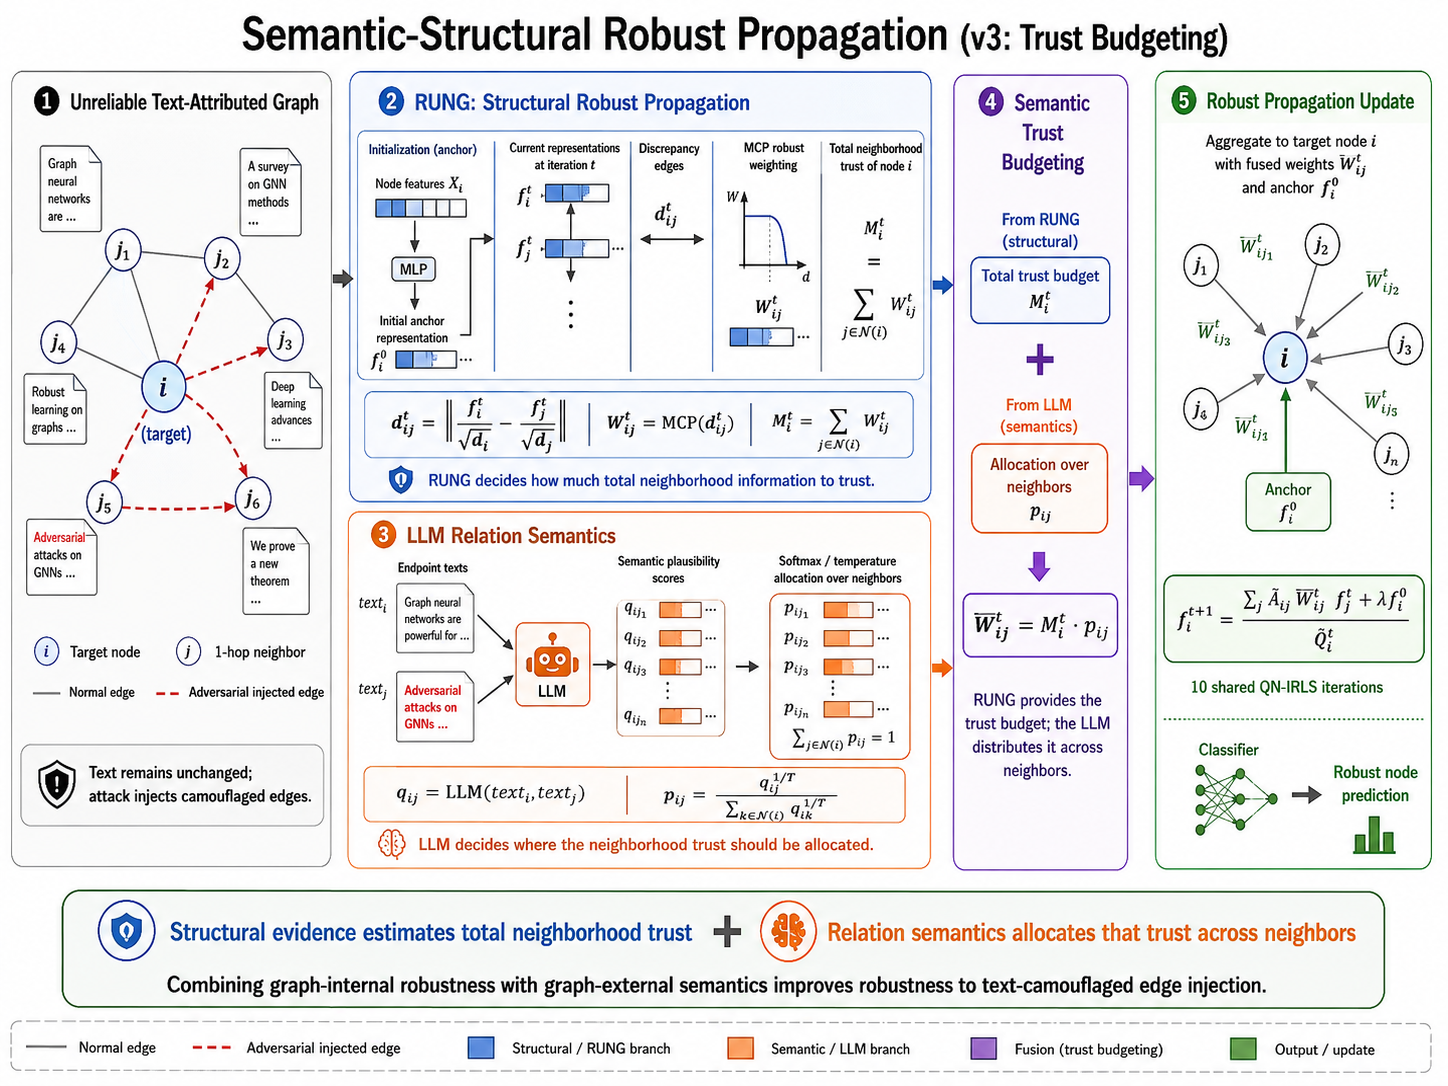
\includegraphics[width=\textwidth]{figures/method_overview.png}
  \caption{Method overview. RUNG uses dynamic graph-internal propagation
  evidence to estimate a node's total neighborhood trust. The LLM reads
  endpoint texts to estimate relation semantics and allocate that trust across
  individual neighbors. The resulting weights are used for anchored robust
  propagation.}
  \label{fig:method-overview}
\end{figure}

For every potential edge $i$--$j$, an LLM reads the endpoint texts and returns
a fixed relation-semantic plausibility score $q_{ij}$. The LLM is evaluated
offline; $q_{ij}$ is frozen during GNN training and propagation.

\subsection{v1: Edge-wise RUNG--LLM Multiplication}

RUNG produces a dynamic structural weight $W_{ij}^t$ for every edge and the
LLM supplies a semantic score $q_{ij}$. v1 combines the two edge by edge:
\[
\overline W_{ij}^t = c_i W_{ij}^t q_{ij},
\]
where $c_i$ is a normalization coefficient intended to avoid unconditional
shrinkage of the total neighborhood weight. A low RUNG weight or a low LLM
score reduces the final edge weight.

\begin{quote}
\textit{v1: RUNG and the LLM both score each edge, then their scores are
multiplied.}
\end{quote}

\subsection{v3: Semantic Trust Budgeting}

RUNG still computes all dynamic edge weights $W_{ij}^t$, but v3 first retains
only their sum for node $i$:
\[
M_i^t = \sum_{j\in N(i)} W_{ij}^t.
\]
This is the current total neighborhood trust estimated from propagation
behavior. The LLM scores are converted into an allocation over the current
neighbors:
\[
p_{ij} = \frac{q_{ij}^{1/T}}
{\sum_{k\in N(i)}q_{ik}^{1/T}}.
\]
The final propagation weight is
\[
\overline W_{ij}^t = M_i^t p_{ij}.
\]
Therefore, RUNG controls how much total information node $i$ accepts from its
current one-hop neighborhood, while the LLM controls how that trust is
distributed among individual neighbors.

\begin{quote}
\textit{v3: RUNG determines the total neighborhood trust; the LLM determines
its edge-wise allocation.}
\end{quote}

\section{Current Results}

All values below are mean $\pm$ standard deviation of node-classification
accuracy (\%) over 12 runs. ``Clean'' is the corresponding accuracy on the
unperturbed graph. Bold denotes the highest mean in each attacked column.

\subsection{Cora}
\begin{center}
\scriptsize
\begin{tabular}{lrrrrrr}
\toprule
Method & Clean & 5\% & 10\% & 20\% & 30\% & 40\% \\
\midrule
GCN & \score{83.3}{0.9} & \score{75.1}{0.8} & \score{70.8}{1.2} & \score{65.0}{1.8} & \score{61.3}{3.1} & \score{58.1}{3.5} \\
GAT & \score{82.9}{0.4} & \score{75.8}{0.3} & \score{71.1}{0.6} & \score{64.9}{0.7} & \score{60.8}{0.4} & \score{57.6}{0.9} \\
APPNP & \score{85.0}{0.6} & \score{75.2}{0.8} & \score{69.1}{1.1} & \score{59.7}{1.7} & \score{52.8}{2.1} & \score{48.6}{2.8} \\
GCN-Jaccard & \score{83.7}{0.3} & \score{74.3}{0.4} & \score{68.6}{0.4} & \score{59.6}{0.5} & \score{52.9}{0.6} & \score{48.1}{0.6} \\
GNNGuard & \score{83.3}{0.6} & \score{76.1}{1.0} & \score{71.0}{0.6} & \score{63.1}{1.1} & \score{57.0}{0.9} & \score{51.8}{0.5} \\
RGCN & \score{85.2}{0.4} & \score{77.0}{0.4} & \score{71.9}{0.4} & \score{63.8}{0.5} & \score{57.2}{0.5} & \score{52.2}{0.7} \\
SCAD & \score{83.6}{0.4} & \score{73.0}{1.2} & \score{65.0}{2.3} & \score{54.2}{3.0} & \score{45.9}{3.0} & \score{41.7}{4.0} \\
TWIRLS & \score{84.3}{1.0} & \score{77.2}{1.1} & \score{73.3}{1.3} & \score{68.2}{2.0} & \score{64.0}{3.0} & \score{61.7}{4.0} \\
GraphSAGE & \score{83.1}{0.2} & \score{74.6}{0.4} & \score{69.6}{0.7} & \score{62.7}{1.2} & \score{57.9}{1.8} & \score{54.2}{2.6} \\
GRAND & \score{83.0}{0.4} & \score{71.9}{0.6} & \score{65.3}{1.1} & \score{54.0}{1.2} & \score{44.9}{1.3} & \score{36.9}{1.5} \\
H2GCN & \score{82.8}{0.3} & \score{74.6}{0.2} & \score{70.4}{0.2} & \score{64.7}{0.8} & \score{60.6}{1.4} & \score{57.6}{1.7} \\
RUNG & \score{84.3}{1.1} & \score{77.7}{1.0} & \score{73.5}{1.2} & \score{68.1}{1.9} & \score{64.6}{2.8} & \score{62.4}{3.6} \\
RUNG + cosine & \score{82.7}{1.3} & \score{75.2}{1.5} & \score{71.1}{1.4} & \score{65.1}{2.4} & \score{63.0}{2.7} & \score{60.5}{4.2} \\
RUNG + SBERT & \score{83.1}{1.2} & \score{76.6}{1.2} & \score{73.4}{1.1} & \score{69.0}{1.5} & \score{66.1}{2.2} & \score{64.1}{3.0} \\
v1: RUNG + LLM & \score{83.4}{1.1} & \score{77.3}{1.2} & \score{74.3}{1.5} & \score{70.4}{2.0} & \score{68.6}{2.8} & \score{66.5}{3.0} \\
\textbf{v3: Trust Budget} & \score{82.7}{0.9} & \textbf{\score{79.6}{1.2}} & \textbf{\score{77.7}{1.4}} & \textbf{\score{75.0}{1.9}} & \textbf{\score{73.2}{2.5}} & \textbf{\score{71.8}{3.1}} \\
\bottomrule
\end{tabular}
\end{center}

\subsection{Citeseer}
\begin{center}
\scriptsize
\begin{tabular}{lrrrrrr}
\toprule
Method & Clean & 5\% & 10\% & 20\% & 30\% & 40\% \\
\midrule
GCN & \score{74.3}{1.1} & \score{67.5}{1.2} & \score{63.9}{1.6} & \score{58.4}{2.2} & \score{54.9}{3.0} & \score{52.2}{3.9} \\
GAT & \score{74.6}{0.6} & \score{70.8}{1.1} & \score{67.4}{1.1} & \score{63.3}{2.1} & \score{60.4}{3.0} & \score{57.4}{4.0} \\
APPNP & \score{74.4}{1.2} & \score{66.6}{1.2} & \score{62.4}{1.3} & \score{56.9}{1.3} & \score{53.1}{1.9} & \score{50.1}{2.1} \\
GCN-Jaccard & \score{75.3}{0.2} & \score{68.7}{0.2} & \score{64.2}{0.3} & \score{57.9}{0.4} & \score{53.1}{0.5} & \score{49.1}{0.4} \\
GNNGuard & \score{75.2}{0.4} & \score{69.9}{0.6} & \score{65.6}{0.6} & \score{59.3}{0.8} & \score{54.5}{0.7} & \score{50.8}{0.9} \\
RGCN & \score{75.7}{0.6} & \score{69.6}{0.5} & \score{65.1}{0.6} & \score{58.8}{0.6} & \score{53.5}{0.6} & \score{49.3}{0.8} \\
SCAD & \score{73.2}{1.0} & \score{65.3}{1.4} & \score{61.2}{1.7} & \score{55.6}{2.2} & \score{51.8}{2.4} & \score{48.6}{2.6} \\
TWIRLS & \score{74.5}{1.2} & \score{68.3}{1.2} & \score{65.0}{1.2} & \score{61.2}{1.6} & \score{58.8}{1.0} & \score{57.7}{1.1} \\
GraphSAGE & \score{70.7}{0.4} & \score{63.2}{0.8} & \score{58.2}{1.1} & \score{51.0}{2.1} & \score{45.8}{2.9} & \score{41.3}{3.6} \\
GRAND & \score{69.3}{0.8} & \score{59.7}{0.6} & \score{53.5}{0.6} & \score{44.6}{1.1} & \score{37.9}{1.6} & \score{31.9}{1.8} \\
H2GCN & \score{71.5}{0.4} & \score{66.2}{0.8} & \score{63.1}{1.6} & \score{59.4}{1.4} & \score{56.8}{2.0} & \score{55.0}{1.8} \\
RUNG & \score{74.4}{1.1} & \score{68.5}{1.1} & \score{65.1}{1.3} & \score{61.7}{1.2} & \score{59.6}{1.3} & \score{58.3}{1.5} \\
RUNG + cosine & \score{74.1}{0.9} & \score{68.2}{1.0} & \score{65.2}{1.1} & \score{61.2}{1.7} & \score{58.9}{2.4} & \score{57.2}{3.2} \\
RUNG + SBERT & \score{74.6}{1.0} & \score{69.2}{0.9} & \score{66.1}{1.1} & \score{62.5}{1.3} & \score{60.5}{1.8} & \score{59.0}{2.1} \\
v1: RUNG + LLM & \score{74.5}{1.4} & \score{69.4}{1.5} & \score{66.9}{1.6} & \score{63.7}{2.1} & \score{61.6}{2.5} & \score{60.4}{2.9} \\
\textbf{v3: Trust Budget} & \score{73.6}{0.9} & \textbf{\score{71.5}{0.9}} & \textbf{\score{70.2}{0.9}} & \textbf{\score{68.6}{1.0}} & \textbf{\score{67.3}{1.1}} & \textbf{\score{66.3}{1.2}} \\
\bottomrule
\end{tabular}
\end{center}

\subsection{WikiCS}
\begin{center}
\scriptsize
\begin{tabular}{lrrrrrr}
\toprule
Method & Clean & 5\% & 10\% & 20\% & 30\% & 40\% \\
\midrule
GCN & \score{79.3}{0.7} & \score{61.5}{1.0} & \score{58.7}{1.3} & \score{56.6}{1.1} & \score{55.2}{1.3} & \score{54.7}{1.1} \\
APPNP & \score{79.4}{0.7} & \score{66.5}{0.9} & \score{64.2}{0.9} & \score{62.3}{1.1} & \score{61.5}{1.2} & \score{61.3}{1.0} \\
SCAD & \score{78.4}{0.7} & \score{62.3}{1.5} & \score{58.8}{1.7} & \score{55.5}{1.6} & \score{54.0}{2.0} & \score{52.9}{1.9} \\
TWIRLS & \score{79.2}{0.7} & \score{70.2}{0.9} & \score{68.3}{0.8} & \score{66.7}{1.0} & \score{65.8}{0.9} & \score{65.4}{1.1} \\
GraphSAGE & \score{79.3}{0.6} & \score{68.1}{1.0} & \score{65.0}{1.1} & \score{62.1}{1.4} & \score{60.8}{1.5} & \score{59.7}{1.4} \\
GRAND & \score{79.0}{0.5} & \score{63.2}{1.2} & \score{58.6}{1.1} & \score{54.0}{1.2} & \score{51.6}{1.3} & \score{49.9}{1.2} \\
H2GCN & \score{79.7}{0.3} & \score{70.1}{0.8} & \score{67.8}{1.0} & \score{65.6}{1.1} & \score{64.6}{0.7} & \score{63.7}{1.0} \\
RUNG & \score{79.1}{0.7} & \score{70.2}{0.8} & \score{68.5}{0.6} & \score{66.9}{0.9} & \score{66.0}{1.1} & \score{65.5}{1.1} \\
RUNG + cosine & \score{79.3}{0.6} & \score{70.2}{0.9} & \score{68.4}{1.0} & \score{66.6}{1.1} & \score{66.1}{1.2} & \score{65.6}{1.3} \\
RUNG + SBERT & \score{79.7}{0.7} & \score{71.1}{0.8} & \score{69.4}{0.8} & \score{68.0}{0.9} & \score{67.5}{0.7} & \score{66.9}{0.9} \\
v1: RUNG + LLM & \score{80.1}{0.5} & \score{74.0}{0.7} & \score{72.6}{0.6} & \score{71.4}{0.7} & \score{70.9}{0.9} & \score{70.7}{0.8} \\
\textbf{v3: Trust Budget} & \score{79.2}{0.6} & \textbf{\score{75.7}{0.6}} & \textbf{\score{75.0}{0.6}} & \textbf{\score{74.3}{0.8}} & \textbf{\score{74.0}{0.8}} & \textbf{\score{73.7}{0.8}} \\
\bottomrule
\end{tabular}
\end{center}


\section{Current Takeaways}

The current v3 RUNG plus LLM trust-budget mechanism is strongest at every evaluated attack
budget on all three datasets. It trades a modest amount of clean accuracy on
Cora and Citeseer for substantially stronger attacked accuracy. The present
scope is text-camouflaged, add-only, white-box edge injection; scalability and
broader evaluation remain open questions.

\section{Next Steps}

\paragraph{Direction 1: Method.}
Understand and refine every component of the current RUNG plus LLM-based
semantic trust-budget mechanism; identify and reduce the clean-accuracy cost of v3; and
develop a path to large graphs, including lower-cost semantic scoring and
teacher--student distillation.

\paragraph{Direction 2: Evaluation.}
Systematically review recent robust-GNN baselines, identify the strongest
missing comparisons, and investigate more realistic robustness settings where
the combination of graph-internal structural evidence and external relation
semantics is genuinely necessary.

\paragraph{Related, separate investigation.}
A parallel, self-contained investigation on the STEM-GNN pretrain/finetune
codebase (a different backbone and evaluation protocol from the RUNG/LLM
setting here) explores a related but distinct question: bounding the
Lipschitz constant of the GNN \emph{encoder} itself, rather than combining
structural and semantic trust signals at the propagation layer. See
\texttt{STEM-GNN/results/encoder\_lipschitz\_reg.tex} for that memo; its
results are not merged into this paper's tables since the two use
different backbones, tasks, and baselines.

\section{Adaptive Robustness Experiments}

All values are mean $\pm$ standard deviation of node-classification accuracy
(\%) over 12 runs. Bold denotes the highest mean in each attacked column for
each dataset.

% ─────────────────────────────────────────────────────────────────────────────
\subsection{Experiment 1: Semantic-Aware Adaptive Attack}
\label{sec:exp1}

We restrict the PGD attacker to the top-$p$\% of the BM25 candidate pool,
ranked by relevance score $q_{ij}$, with $p \in \{100, 75, 50, 25\}$\%.
At $p{=}100\%$ the attacker has full access to all semantic candidates.

\paragraph{All methods at $p{=}100\%$.}
On Cora and WikiCS, v3 (Trust Budget) is the most robust method at every
budget. On CiteSeer, H2GCN unexpectedly outperforms v3 across all attack
budgets — a method with ego-network separation that appears to be harder
to attack via semantic edge injection on this graph.

\begin{center}
\scriptsize
\begin{tabular}{lrrrrrr}
\toprule
Method & Clean & 5\% & 10\% & 20\% & 30\% & 40\% \\
\midrule
\multicolumn{7}{l}{\textit{Cora}} \\
\midrule
GCN            & \score{83.0}{0.9} & \score{75.0}{0.9} & \score{70.8}{1.2} & \score{65.2}{2.0} & \score{61.5}{2.8} & \score{58.8}{3.6} \\
GNNGuard       & \score{83.5}{0.9} & \score{75.5}{0.8} & \score{71.8}{1.0} & \score{66.8}{1.8} & \score{63.7}{2.8} & \score{61.8}{3.4} \\
GCN-Jaccard    & \score{83.0}{0.9} & \score{75.0}{0.9} & \score{70.8}{1.2} & \score{65.2}{2.0} & \score{61.5}{2.8} & \score{58.8}{3.6} \\
SCAD           & \score{83.7}{0.6} & \score{72.5}{2.1} & \score{65.1}{3.0} & \score{54.4}{3.9} & \score{46.8}{5.0} & \score{42.1}{5.0} \\
APPNP          & \score{85.0}{0.5} & \score{74.9}{0.6} & \score{68.4}{0.9} & \score{58.4}{1.4} & \score{51.8}{2.2} & \score{47.1}{2.0} \\
TWIRLS         & \score{83.8}{1.2} & \score{76.9}{1.3} & \score{73.4}{1.4} & \score{68.5}{1.7} & \score{65.7}{2.3} & \score{63.9}{2.9} \\
H2GCN          & \score{81.4}{0.7} & \score{74.7}{0.8} & \score{71.7}{1.1} & \score{68.1}{2.0} & \score{65.9}{2.4} & \score{64.6}{2.6} \\
GraphSAGE      & \score{81.4}{1.0} & \score{74.4}{1.2} & \score{71.0}{1.5} & \score{67.0}{2.7} & \score{64.5}{3.6} & \score{62.8}{4.0} \\
GRAND          & \score{82.5}{0.9} & \score{73.9}{0.9} & \score{68.9}{0.9} & \score{61.3}{1.4} & \score{55.5}{2.0} & \score{50.9}{2.3} \\
RUNG           & \score{83.5}{1.6} & \score{76.4}{1.6} & \score{72.9}{1.8} & \score{67.9}{2.2} & \score{64.5}{2.8} & \score{62.5}{3.4} \\
\textbf{v3 (Trust Budget)} & \score{82.0}{1.4} & \textbf{\score{79.0}{1.6}} & \textbf{\score{77.2}{1.9}} & \textbf{\score{74.7}{2.3}} & \textbf{\score{72.9}{2.8}} & \textbf{\score{71.6}{2.9}} \\
\midrule
\multicolumn{7}{l}{\textit{CiteSeer}} \\
\midrule
GCN            & \score{74.2}{0.9} & \score{67.7}{1.0} & \score{64.0}{1.1} & \score{59.1}{1.3} & \score{55.8}{1.6} & \score{53.4}{2.0} \\
GNNGuard       & \score{73.8}{1.1} & \score{67.3}{1.2} & \score{63.5}{1.5} & \score{58.6}{1.7} & \score{55.3}{2.0} & \score{53.0}{2.5} \\
GCN-Jaccard    & \score{74.2}{0.9} & \score{67.7}{1.0} & \score{64.0}{1.1} & \score{59.1}{1.3} & \score{55.8}{1.6} & \score{53.4}{2.0} \\
SCAD           & \score{73.5}{1.2} & \score{64.8}{1.3} & \score{60.1}{2.0} & \score{54.7}{2.8} & \score{50.5}{3.8} & \score{46.5}{4.6} \\
APPNP          & \score{73.8}{1.1} & \score{65.8}{1.6} & \score{61.6}{2.7} & \score{55.8}{3.7} & \score{51.5}{4.5} & \score{48.4}{5.1} \\
TWIRLS         & \score{74.0}{1.3} & \score{68.0}{1.3} & \score{64.8}{1.6} & \score{60.8}{2.0} & \score{58.3}{2.7} & \score{56.8}{3.3} \\
\textbf{H2GCN} & \score{72.6}{1.2} & \textbf{\score{71.7}{1.0}} & \textbf{\score{71.3}{1.1}} & \textbf{\score{70.6}{2.4}} & \textbf{\score{70.3}{3.1}} & \textbf{\score{70.1}{3.4}} \\
GraphSAGE      & \score{72.3}{1.3} & \score{70.8}{2.3} & \score{70.0}{3.1} & \score{68.7}{5.3} & \score{68.1}{6.4} & \score{67.6}{7.3} \\
GRAND          & \score{71.2}{1.0} & \score{69.5}{2.3} & \score{69.0}{2.9} & \score{66.2}{6.5} & \score{64.7}{8.8} & \score{63.4}{10.7} \\
RUNG           & \score{74.4}{1.0} & \score{68.2}{1.3} & \score{64.9}{1.7} & \score{60.6}{2.4} & \score{57.9}{3.2} & \score{56.2}{4.1} \\
v3 (Trust Budget) & \score{73.3}{1.0} & \score{71.3}{1.0} & \score{70.1}{1.1} & \score{68.4}{1.1} & \score{67.0}{1.3} & \score{66.0}{1.2} \\
\midrule
\multicolumn{7}{l}{\textit{WikiCS}} \\
\midrule
GCN            & \score{79.3}{0.7} & \score{61.3}{1.2} & \score{58.7}{1.3} & \score{56.4}{1.5} & \score{55.2}{1.3} & \score{54.6}{1.4} \\
SCAD           & \score{78.4}{0.8} & \score{62.7}{1.5} & \score{58.5}{1.6} & \score{55.2}{2.0} & \score{53.8}{2.3} & \score{53.0}{2.5} \\
APPNP          & \score{79.3}{0.6} & \score{66.2}{0.8} & \score{64.3}{1.0} & \score{62.4}{1.1} & \score{61.8}{0.9} & \score{61.2}{1.2} \\
TWIRLS         & \score{79.3}{0.8} & \score{70.2}{0.9} & \score{68.3}{1.0} & \score{66.5}{1.2} & \score{66.1}{1.0} & \score{65.5}{1.1} \\
RUNG           & \score{79.2}{0.8} & \score{70.2}{1.1} & \score{68.5}{0.9} & \score{66.9}{0.9} & \score{66.2}{1.2} & \score{65.8}{1.0} \\
\textbf{v3 (Trust Budget)} & \score{79.3}{0.7} & \textbf{\score{75.8}{0.8}} & \textbf{\score{75.1}{0.7}} & \textbf{\score{74.3}{0.7}} & \textbf{\score{73.9}{0.7}} & \textbf{\score{73.7}{0.8}} \\
\bottomrule
\end{tabular}
\end{center}

\paragraph{Pool-fraction sensitivity (RUNG and v3).}
Reducing the attack pool forces the attacker to use lower-quality candidate
edges. RUNG recovers substantially as $p$ decreases (e.g.\ Cora
62.5\%$\to$75.7\% at $\epsilon{=}0.40$), while v3's gain is more modest
(71.6\%$\to$77.4\%), confirming that v3's trust budget makes it less dependent
on pool quality.

\begin{center}
\scriptsize
\begin{tabular}{lrrrrrr}
\toprule
Method & Clean & 5\% & 10\% & 20\% & 30\% & 40\% \\
\midrule
\multicolumn{7}{l}{\textit{Cora}} \\
\midrule
RUNG, $p{=}100\%$ & \score{83.5}{1.6} & \score{76.4}{1.6} & \score{72.9}{1.8} & \score{67.9}{2.2} & \score{64.5}{2.8} & \score{62.5}{3.4} \\
RUNG, $p{=}75\%$  & \score{83.5}{1.6} & \score{77.1}{1.6} & \score{73.7}{1.7} & \score{69.3}{1.9} & \score{66.8}{2.4} & \score{65.1}{3.0} \\
RUNG, $p{=}50\%$  & \score{83.5}{1.6} & \score{78.2}{1.5} & \score{75.7}{1.6} & \score{72.8}{1.9} & \score{71.2}{2.0} & \score{70.1}{2.1} \\
RUNG, $p{=}25\%$  & \score{83.5}{1.6} & \score{80.1}{1.3} & \score{78.9}{1.3} & \score{77.3}{1.5} & \score{76.3}{1.5} & \score{75.7}{1.6} \\
\addlinespace
v3, $p{=}100\%$   & \score{82.0}{1.4} & \score{79.0}{1.6} & \score{77.2}{1.9} & \score{74.7}{2.3} & \score{72.9}{2.8} & \score{71.6}{2.9} \\
v3, $p{=}75\%$    & \score{82.0}{1.4} & \score{79.2}{1.6} & \score{77.4}{1.9} & \score{75.0}{2.4} & \score{73.2}{2.7} & \score{72.2}{2.9} \\
v3, $p{=}50\%$    & \score{82.0}{1.4} & \score{79.6}{1.5} & \score{78.2}{1.7} & \score{76.3}{2.1} & \score{75.1}{2.4} & \score{74.2}{2.5} \\
v3, $p{=}25\%$    & \score{82.0}{1.4} & \score{80.5}{1.5} & \score{79.7}{1.6} & \score{78.7}{1.6} & \score{78.0}{1.8} & \score{77.4}{1.7} \\
\midrule
\multicolumn{7}{l}{\textit{CiteSeer}} \\
\midrule
RUNG, $p{=}100\%$ & \score{74.4}{1.0} & \score{68.2}{1.3} & \score{64.9}{1.7} & \score{60.6}{2.4} & \score{57.9}{3.2} & \score{56.2}{4.1} \\
RUNG, $p{=}75\%$  & \score{74.4}{1.0} & \score{68.8}{1.2} & \score{66.0}{1.4} & \score{62.3}{2.3} & \score{60.3}{3.1} & \score{58.9}{3.7} \\
RUNG, $p{=}50\%$  & \score{74.4}{1.0} & \score{69.9}{1.2} & \score{67.6}{1.4} & \score{65.2}{2.1} & \score{63.9}{2.5} & \score{63.1}{2.7} \\
RUNG, $p{=}25\%$  & \score{74.4}{1.0} & \score{69.9}{1.2} & \score{67.6}{1.4} & \score{65.2}{2.1} & \score{63.9}{2.5} & \score{63.1}{2.7} \\
\addlinespace
v3, $p{=}100\%$   & \score{73.3}{1.0} & \score{71.3}{1.0} & \score{70.1}{1.1} & \score{68.4}{1.1} & \score{67.0}{1.3} & \score{66.0}{1.2} \\
v3, $p{=}75\%$    & \score{73.3}{1.0} & \score{71.4}{1.1} & \score{70.2}{1.0} & \score{68.7}{1.1} & \score{67.6}{1.1} & \score{66.7}{1.2} \\
v3, $p{=}50\%$    & \score{73.3}{1.0} & \score{71.6}{1.0} & \score{70.7}{1.0} & \score{69.5}{1.1} & \score{68.6}{1.1} & \score{68.1}{1.2} \\
v3, $p{=}25\%$    & \score{73.5}{0.8} & \score{71.8}{0.8} & \score{70.9}{0.7} & \score{69.5}{1.1} & \score{68.7}{1.4} & \score{68.1}{1.2} \\
\midrule
\multicolumn{7}{l}{\textit{WikiCS}} \\
\midrule
RUNG, $p{=}100\%$ & \score{79.2}{0.8} & \score{70.2}{1.1} & \score{68.5}{0.9} & \score{66.9}{0.9} & \score{66.2}{1.2} & \score{65.8}{1.0} \\
RUNG, $p{=}75\%$  & \score{79.1}{0.6} & \score{71.9}{0.8} & \score{70.6}{1.0} & \score{69.5}{0.9} & \score{68.6}{0.9} & \score{68.2}{1.1} \\
RUNG, $p{=}50\%$  & \score{79.2}{0.7} & \score{71.9}{0.9} & \score{70.5}{0.8} & \score{69.2}{1.1} & \score{68.7}{0.8} & \score{68.3}{1.0} \\
RUNG, $p{=}25\%$  & \score{79.2}{0.8} & \score{75.1}{0.8} & \score{74.2}{0.7} & \score{73.7}{0.9} & \score{73.3}{1.0} & \score{73.3}{1.0} \\
\addlinespace
v3, $p{=}100\%$   & \score{79.3}{0.7} & \score{75.8}{0.8} & \score{75.1}{0.7} & \score{74.3}{0.7} & \score{73.9}{0.7} & \score{73.7}{0.8} \\
v3, $p{=}75\%$    & \score{79.2}{0.6} & \score{75.9}{0.7} & \score{75.3}{0.7} & \score{74.7}{0.6} & \score{74.4}{0.6} & \score{74.2}{0.7} \\
v3, $p{=}50\%$    & \score{79.3}{0.7} & \score{75.9}{0.7} & \score{75.1}{0.8} & \score{74.5}{0.7} & \score{74.2}{0.7} & \score{74.1}{0.6} \\
v3, $p{=}25\%$    & \score{79.2}{0.8} & \textbf{\score{76.7}{0.9}} & \textbf{\score{76.4}{0.7}} & \textbf{\score{76.1}{0.7}} & \textbf{\score{75.8}{0.7}} & \textbf{\score{75.9}{0.8}} \\
\bottomrule
\end{tabular}
\end{center}


% ─────────────────────────────────────────────────────────────────────────────
\subsection{Experiment 2: Scorer Quality Ablation}
\label{sec:exp2}

We fix $p{=}100\%$ and replace the BM25-derived $q_{ij}$ with degraded
scorers: \textbf{LLM oracle} (original BM25); \textbf{Random}
($q_{ij}\!\sim\!\mathcal{U}[0,1]$); \textbf{Noisy}
$\sigma\in\{0.5,1.0,2.0\}$ (BM25 plus $\mathcal{N}(0,\sigma^2)$ noise);
\textbf{Uniform-high} (constant, disabling the budget).

On Cora and CiteSeer, the LLM oracle is the strongest scorer and robustness
degrades gracefully with noise. Notably on Cora, Uniform-high achieves the
highest robustness at $\epsilon{=}0.05$ (79.3\% vs.\ LLM 79.0\%), suggesting
the trust-budget normalisation mechanism itself provides most of the benefit
on this graph, independent of scorer quality. On WikiCS the LLM oracle wins
at every budget. On PubMed, Random scoring slightly outperforms the oracle,
confirming the normalised competition mechanism is the primary driver there.

\begin{center}
\scriptsize
\begin{tabular}{lrrrrrr}
\toprule
Scorer & Clean & 5\% & 10\% & 20\% & 30\% & 40\% \\
\midrule
\multicolumn{7}{l}{\textit{Cora} (victim: v3)} \\
\midrule
LLM oracle           & \score{82.0}{1.4} & \score{79.0}{1.6} & \textbf{\score{77.2}{1.9}} & \textbf{\score{74.7}{2.3}} & \textbf{\score{72.9}{2.8}} & \textbf{\score{71.6}{2.9}} \\
Random               & \score{82.7}{1.2} & \score{78.1}{1.1} & \score{75.3}{1.4} & \score{71.4}{1.7} & \score{68.9}{2.2} & \score{67.1}{2.5} \\
Noisy $\sigma{=}0.5$ & \score{82.3}{1.7} & \score{78.1}{1.6} & \score{75.5}{1.9} & \score{71.8}{2.3} & \score{69.2}{2.7} & \score{67.3}{3.0} \\
Noisy $\sigma{=}1.0$ & \score{82.0}{1.7} & \score{77.7}{1.9} & \score{74.9}{2.3} & \score{71.2}{3.0} & \score{68.6}{3.4} & \score{67.0}{4.1} \\
Noisy $\sigma{=}2.0$ & \score{81.3}{1.9} & \score{76.4}{1.8} & \score{73.4}{1.9} & \score{69.3}{2.5} & \score{66.7}{3.2} & \score{65.1}{3.5} \\
Uniform-high         & \score{83.2}{1.2} & \textbf{\score{79.3}{1.4}} & \score{77.0}{1.7} & \score{73.7}{2.2} & \score{71.6}{2.4} & \score{70.2}{2.5} \\
\midrule
\multicolumn{7}{l}{\textit{CiteSeer} (victim: v3)} \\
\midrule
LLM oracle           & \score{73.3}{1.0} & \textbf{\score{71.3}{1.0}} & \textbf{\score{70.1}{1.1}} & \textbf{\score{68.4}{1.1}} & \textbf{\score{67.0}{1.3}} & \textbf{\score{66.0}{1.2}} \\
Random               & \score{73.8}{1.0} & \score{70.3}{0.9} & \score{68.2}{0.9} & \score{65.6}{1.0} & \score{63.9}{1.0} & \score{62.6}{1.1} \\
Noisy $\sigma{=}0.5$ & \score{73.9}{0.7} & \score{71.4}{0.7} & \score{69.9}{0.7} & \score{68.0}{0.6} & \score{66.6}{0.6} & \score{65.6}{0.6} \\
Noisy $\sigma{=}1.0$ & \score{73.6}{1.2} & \score{70.7}{1.4} & \score{69.1}{1.4} & \score{66.8}{1.7} & \score{65.0}{1.9} & \score{64.0}{1.9} \\
Noisy $\sigma{=}2.0$ & \score{73.4}{1.1} & \score{70.0}{1.0} & \score{67.8}{1.4} & \score{65.0}{2.2} & \score{62.8}{2.4} & \score{62.4}{1.4} \\
Uniform-high         & \score{73.9}{0.9} & \score{70.8}{1.1} & \score{69.0}{1.3} & \score{66.4}{1.6} & \score{64.8}{2.1} & \score{63.4}{2.3} \\
\midrule
\multicolumn{7}{l}{\textit{WikiCS} (victim: v3)} \\
\midrule
LLM oracle           & \score{79.3}{0.7} & \textbf{\score{75.8}{0.8}} & \textbf{\score{75.1}{0.7}} & \textbf{\score{74.3}{0.7}} & \textbf{\score{73.9}{0.7}} & \textbf{\score{73.7}{0.8}} \\
Random               & \score{79.4}{0.6} & \score{73.3}{0.7} & \score{72.2}{0.8} & \score{71.0}{0.9} & \score{70.6}{0.7} & \score{70.4}{0.7} \\
Noisy $\sigma{=}0.5$ & \score{79.4}{0.6} & \score{75.5}{0.7} & \score{74.4}{0.7} & \score{73.8}{0.7} & \score{73.4}{0.8} & \score{73.3}{0.8} \\
Noisy $\sigma{=}1.0$ & \score{79.2}{0.6} & \score{74.8}{0.7} & \score{74.0}{0.7} & \score{73.1}{0.8} & \score{72.8}{0.8} & \score{72.6}{0.8} \\
Noisy $\sigma{=}2.0$ & \score{79.3}{0.7} & \score{74.2}{0.8} & \score{73.3}{0.7} & \score{72.5}{0.8} & \score{71.8}{0.9} & \score{71.7}{0.9} \\
Uniform-high         & \score{79.3}{0.7} & \score{70.3}{1.0} & \score{68.8}{0.9} & \score{67.9}{0.7} & \score{67.3}{0.8} & \score{66.9}{0.8} \\
\midrule
\multicolumn{7}{l}{\textit{PubMed} (victim: v3)} \\
\midrule
LLM oracle           & \score{87.1}{0.3} & \score{79.1}{0.3} & \score{73.5}{0.3} & \score{63.2}{1.0} & \score{55.1}{1.5} & \score{49.7}{1.6} \\
Random               & \score{87.1}{0.3} & \textbf{\score{79.7}{0.3}} & \textbf{\score{74.4}{0.4}} & \textbf{\score{64.8}{1.0}} & \textbf{\score{57.2}{1.4}} & \textbf{\score{51.7}{1.6}} \\
Noisy $\sigma{=}0.5$ & \score{87.2}{0.4} & \score{79.1}{0.4} & \score{73.2}{0.6} & \score{62.6}{1.0} & \score{54.3}{1.1} & \score{48.7}{1.0} \\
Noisy $\sigma{=}1.0$ & \score{87.1}{0.3} & \score{79.0}{0.4} & \score{73.3}{0.6} & \score{62.6}{1.0} & \score{54.3}{1.1} & \score{48.8}{1.0} \\
Noisy $\sigma{=}2.0$ & \score{87.2}{0.4} & \score{79.2}{0.4} & \score{73.3}{0.6} & \score{62.7}{1.0} & \score{54.7}{1.1} & \score{49.3}{1.0} \\
Uniform-high         & \score{87.1}{0.3} & \score{78.6}{0.3} & \score{72.4}{0.4} & \score{60.8}{1.0} & \score{52.6}{1.1} & \score{47.4}{1.1} \\
\bottomrule
\end{tabular}
\end{center}


% ─────────────────────────────────────────────────────────────────────────────
\subsection{Experiment 3: Transfer Attack}
\label{sec:exp3}

The attacker switches to a random-$k{=}20$ pool (20 uniformly sampled
non-edges per node) while models retain their BM25-calibrated defences.

On Cora, v3 (76.2\% at $\epsilon{=}0.05$) remains competitive with the
best baseline (TWIRLS 76.3\%) and outperforms RUNG (75.9\%), unlike the
WikiCS result where v3 falls below RUNG under the random pool. On CiteSeer,
v3 (69.3\%) is the most robust method at every budget. On WikiCS, RUNG
maintains its advantage over v3 under the out-of-distribution pool, and
GCN, SCAD, and APPNP all drop dramatically (e.g.\ GCN: 49.5\% at
$\epsilon{=}0.05$), far below their BM25-pool performance.

\begin{center}\scriptsize\begin{tabular}{lrrrrrr}
\toprule
Method & Clean & 5\% & 10\% & 20\% & 30\% & 40\% \\
\midrule
\multicolumn{7}{l}{\textit{Cora}} \\
\midrule
GCN            & \score{83.0}{0.9} & \score{75.0}{0.9} & \score{70.8}{1.1} & \score{65.2}{1.9} & \score{61.5}{2.7} & \score{58.8}{3.5} \\
GNNGuard       & \score{83.5}{0.9} & \score{75.5}{0.7} & \score{71.8}{1.0} & \score{66.8}{1.8} & \score{63.7}{2.7} & \score{61.8}{3.2} \\
GCN-Jaccard    & \score{83.0}{0.9} & \score{75.0}{0.9} & \score{70.8}{1.1} & \score{65.2}{1.9} & \score{61.5}{2.7} & \score{58.8}{3.5} \\
SCAD           & \score{83.7}{0.6} & \score{72.5}{2.0} & \score{65.1}{2.9} & \score{54.4}{3.8} & \score{46.8}{4.8} & \score{42.1}{4.8} \\
APPNP          & \score{85.0}{0.5} & \score{74.9}{0.6} & \score{68.4}{0.9} & \score{58.7}{1.3} & \score{51.7}{1.9} & \score{47.0}{1.8} \\
TWIRLS         & \score{83.8}{1.2} & \score{76.9}{1.2} & \score{73.4}{1.4} & \score{68.5}{1.6} & \score{65.7}{2.2} & \score{63.9}{2.8} \\
H2GCN          & \score{81.4}{0.7} & \score{74.7}{0.8} & \score{71.7}{1.1} & \score{68.1}{1.9} & \score{65.9}{2.3} & \score{64.6}{2.5} \\
GraphSAGE      & \score{81.4}{0.9} & \score{74.4}{1.2} & \score{71.0}{1.5} & \score{67.0}{2.6} & \score{64.5}{3.4} & \score{62.8}{3.8} \\
GRAND          & \score{82.5}{0.8} & \score{73.9}{0.9} & \score{68.9}{0.9} & \score{61.3}{1.4} & \score{55.5}{1.9} & \score{50.9}{2.2} \\
RUNG           & \score{83.5}{1.5} & \score{76.4}{1.5} & \score{72.9}{1.7} & \score{67.9}{2.1} & \score{64.5}{2.6} & \score{62.5}{3.3} \\
v3 (Trust Budget) & \score{82.0}{1.3} & \textbf{\score{79.0}{1.5}} & \textbf{\score{77.2}{1.8}} & \textbf{\score{74.7}{2.2}} & \textbf{\score{72.9}{2.7}} & \textbf{\score{71.6}{2.7}} \\
\midrule
\multicolumn{7}{l}{\textit{CiteSeer}} \\
\midrule
GCN            & \score{74.2}{0.8} & \score{67.7}{0.9} & \score{64.0}{1.0} & \score{59.1}{1.3} & \score{55.8}{1.5} & \score{53.4}{1.9} \\
GNNGuard       & \score{73.8}{1.1} & \score{67.3}{1.1} & \score{63.5}{1.4} & \score{58.6}{1.6} & \score{55.3}{2.0} & \score{53.0}{2.4} \\
GCN-Jaccard    & \score{74.2}{0.8} & \score{67.7}{0.9} & \score{64.0}{1.0} & \score{59.1}{1.3} & \score{55.8}{1.5} & \score{53.4}{1.9} \\
SCAD           & \score{73.4}{1.1} & \score{64.8}{1.3} & \score{60.1}{1.9} & \score{54.7}{2.7} & \score{50.5}{3.6} & \score{46.5}{4.4} \\
APPNP          & \score{73.8}{1.0} & \score{65.8}{1.6} & \score{61.6}{2.6} & \score{55.8}{3.5} & \score{51.5}{4.3} & \score{48.4}{4.9} \\
TWIRLS         & \score{74.0}{1.2} & \score{68.0}{1.3} & \score{64.8}{1.6} & \score{60.8}{2.0} & \score{58.3}{2.6} & \score{56.8}{3.2} \\
H2GCN          & \score{72.6}{1.2} & \textbf{\score{71.7}{0.9}} & \textbf{\score{71.3}{1.1}} & \textbf{\score{70.6}{2.3}} & \textbf{\score{70.3}{3.0}} & \textbf{\score{70.1}{3.3}} \\
GraphSAGE      & \score{72.3}{1.3} & \score{70.8}{2.2} & \score{70.0}{3.0} & \score{68.7}{5.1} & \score{68.1}{6.2} & \score{67.6}{7.0} \\
GRAND          & \score{71.2}{1.0} & \score{69.5}{2.2} & \score{69.0}{2.8} & \score{66.2}{6.2} & \score{64.7}{8.5} & \score{63.4}{10.3} \\
RUNG           & \score{74.4}{1.0} & \score{68.2}{1.2} & \score{64.9}{1.6} & \score{60.6}{2.3} & \score{57.9}{3.1} & \score{56.2}{3.9} \\
v3 (Trust Budget) & \score{73.3}{0.9} & \score{71.3}{1.0} & \score{70.1}{1.0} & \score{68.4}{1.1} & \score{67.0}{1.2} & \score{66.0}{1.1} \\
\midrule
\multicolumn{7}{l}{\textit{WikiCS}} \\
\midrule
GCN            & \score{79.3}{0.7} & \score{61.3}{1.1} & \score{58.7}{1.2} & \score{56.4}{1.4} & \score{55.2}{1.2} & \score{54.6}{1.4} \\
SCAD           & \score{78.5}{0.7} & \score{62.7}{1.4} & \score{58.5}{1.5} & \score{55.2}{1.9} & \score{53.8}{2.2} & \score{53.0}{2.3} \\
APPNP          & \score{79.4}{0.7} & \score{66.2}{0.8} & \score{64.3}{0.9} & \score{62.4}{1.0} & \score{61.8}{0.9} & \score{61.2}{1.1} \\
TWIRLS         & \score{79.2}{0.8} & \score{70.2}{0.8} & \score{68.3}{1.0} & \score{66.5}{1.1} & \score{66.1}{1.0} & \score{65.5}{1.0} \\
RUNG           & \score{79.2}{0.7} & \score{70.2}{1.0} & \score{68.5}{0.9} & \score{66.9}{0.9} & \score{66.2}{1.2} & \score{65.8}{1.0} \\
v3 (Trust Budget) & \score{79.3}{0.6} & \textbf{\score{75.8}{0.7}} & \textbf{\score{75.1}{0.7}} & \textbf{\score{74.3}{0.7}} & \textbf{\score{73.9}{0.7}} & \textbf{\score{73.7}{0.7}} \\
\bottomrule
\end{tabular}\end{center}


\end{document}
